  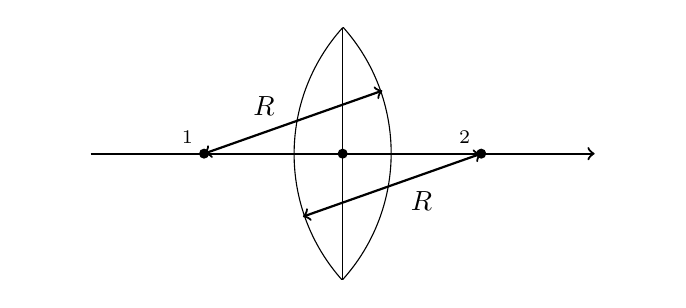
\begin{tikzpicture}[scale=0.8]
    \clip (-5,-2) rectangle (5,2) ; %Les dimensions de l'image

    \draw [->,thick] (-4,0) -- (4,0) ; %% L'axe optique

   \filldraw [black] (0,0) circle (2pt) node [above right] {$\ptO$} ;  %Le centre optique
   
   \filldraw [black] (-2.2,0) circle (2pt) node [above left] {$\ptC_1$} ;  %Le centre du rayon de courbure
   
   \filldraw [black] (2.2,0) circle (2pt) node [above left] {$\ptC_2$} ;  %Le centre du second rayon de courbure

    \draw (0,2) arc (138:222:3) ;
    \draw (0,-2) arc (-42:42:3) ;  %Lentille biconvexe
    
    \draw [-,thin] (0,-2) -- (0,2) ; %% L'axe de la lentille
    
    \draw [<->,thick] (-2.2,0) -- (0.63,1) ; %% Repérage rayon de courbure 1
    \draw node at (-1.25,0.75) {$R$} ;
    
    \draw [<->,thick] (2.2,0) -- (-0.63,-1) ; %% Repérage rayon de courbure 2
    \draw node at (1.25,-0.75) {$R$} ;
      
  \end{tikzpicture}